\chapter{Begin}
    \section{Who did this}
    \tab Sometimes saying thank you is important, this book have the name and the heart of a group, full of disagreements. We are \textbf{different} and that is what makes us \textbf{strong}. Believe in yourself, and when u can't, believe in the people which are in your side.

    Thank you.

    Here is a list of names which contributed to build this book (for those who are asking, it was sorted by random\_shuffle  in C++20 using srand(252)):
    \begin{itemize}
        \item Lesin
        \item Alunea
        \item Nopebi Lifesa
        \item Atak Kichan
        \item Faslecar
        \item Nollyad
        \item Laelovatsug
        \item Ognol Tohberum
        \item Nhotivew
    \end{itemize}
    \section{tips}
    \begin{itemize}
    \item Remember that binary lifting isn't just for trees.
    
    \item Expected value? contribution is the way.
    
    \item DP? maybe a slow solution can be optimized.
    
    \item Chill, the contest is long, starting slow is good...
    
    \item Breath, drink water, make jokes, eat chocolate, at the end, have fun with your friends.
    
    \item A Greedy is a risk, but can be done. No one knows how to proof this shit anyway...
    \item flow? is this bipartite?
    \item remember what u can do in bipartite graphs:
    \begin{itemize}
        \item minimum vertex cover = maximum matching
        \item clique maximum(same as previous one) 
        \item maximum independent set = complement of minimum vertex cover
    \end{itemize}
    
    \item Remember, a binary search can simplify a lot!

    \item Can you model any recurrence?

    \item Write alot, Think out, Text.

    \item Don't be fixed in finding a fast solution, find one solution, and then, try to understand it.

    \item are there modulus? maybe splitting in cases can help.

    \item is this monotonic(increasing or decreasing)?
    
    \item Geometry has 4 options: Line sweep, binary search, Convex hull and Math.

    \item Game theory? just brute. recurrence in big num? just brute. Overall bruting is gud.
    
    \item BREATH!
    
    \item Your friends are here to help!!!
    
    \item Hug each other, spread love, not war.
    
    \item A funny joke doesn't have to offend a friend.
    
    \item YOU ARE A TEAM!!!

    \item idk maybe guessing that only checking primes is enough(if it doesn't work, try with powers of two)

    \item if u can't do $n \log$, just do $n\log^2$ u bitch
    
    \item remember, you can do some factorial stuff using convolutions.
    
    \end{itemize}
    
    % \newpage

    % \section{coisas pra fazer na lib}

    % \begin{itemize}
    %     \item Padronizar os códigos de geometria;
    %     \item Fazer o BigInt com Karatsuba;
    %     \item Convolução de Teoria dos Números;
    %     \item Colocar a nova Treap;
    % \end{itemize}

    \newpage
    \section{template - makefile - terminaltricks}
    \lstinputlisting{./solutions/template.cpp} 

    \lstinputlisting{./solutions/makefile}
    \lstinputlisting{./solutions/terminaltrick} 
    \newpage
    \section{math formulas}
    \begin{itemize}
        \item $a_n = a_{n-1} + r$
        \item $a_n = a_1 + (n-1)*r$
        \item \begin{Large}
            $soma_{(l,r)} = \frac{(a_l + a_r) * (r-l+1)}{2}$
        \end{Large}
    \end{itemize}

    \begin{itemize}
    \item $a_n = a_{n-1}*q$
    \item $a_n = a_1*q^{n-1}$
    \item \begin{Large}
            $soma_{(l,r)} = \frac{a_l  * (q^{(r-l+1)}-1)}{q-1}$
        \end{Large}
    \end{itemize}
     
    \textit{Fórmula de Heron para Triângulos:} $\sqrt{p\cdot (p-b) \cdot (p-c) \cdot (p-d)}$
    
    \textit{Fórmula de Heron para Quadriláteros:}
    
    \begin{itemize}
        \item $p = (a+b+c+d)/2$
        \item $A = \sqrt{(p-a) \cdot (p-b) \cdot (p-c) \cdot (p-d)}$
        \item $A \rightarrow$ Maior área formada por 4 lados de um quadrilátero.
    \end{itemize}

    \textit{Lagrange Multipliers:}

    We want to optimize a function $f(x_1,x_2,\dots,x_n)$ subject to the constraints
    $ g_i(x_1,x_2,\dots,x_n) = k_i$ where $1 \le i \le m$ and $m$ is the number of constraints, to solve it, we use the Method of Lagrange Multipliers. It consists in solving the following system of equations:

        \[
            \left\{
            \begin{array}{{rcl}}
               \nabla f(x_1,x_2,\dots,x_n) & = & \sum_{i=1}^{m} \lambda_i \nabla g_i(x_1,x_2,\dots,x_n)  \\
                g_i(x_1,x_2,\dots,x_n)     & = & k_i \ \ \ \ \ \ \ \text{for $1 \le i \le m$}
            \end{array}
            \right.
        \]
    
    For the first equation, you derivate for each variable and solve for each derivation.
    
    \begin{figure}[ht]
    \begin{center}
    \begin{minipage}{.48\textwidth}
        \centering
        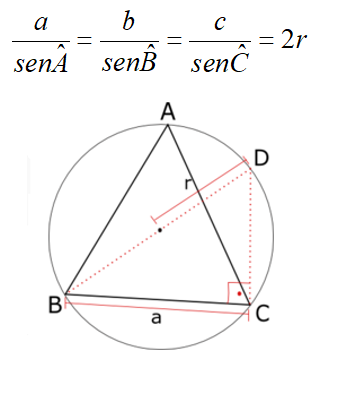
\includegraphics[scale=0.7]{imgs/leidossenos.png}
        \captionof{figure}{Lei dos senos}
    \end{minipage}
    \begin{minipage}{.48\textwidth}
    \centering
        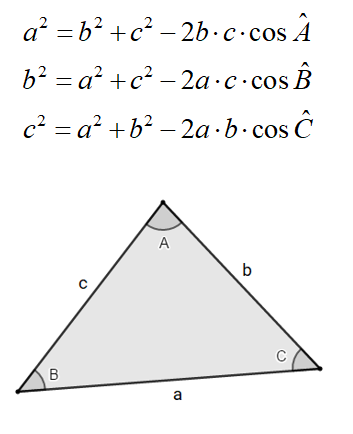
\includegraphics[scale=0.7]{imgs/leidoscosenos.png}
        \captionof{figure}{Lei dos cossenos}
    \end{minipage}
    \end{center}
    \end{figure}
    \section{Stress Test}
    \tab During the contest, sometimes u will need to stress test an solution.
    the steps are:
    \begin{itemize}
        \item Code a Brute Force(do as lazy as possible, focus in not spend time coding it)
        \item Code a generator (in the following lines there are some generators for vectors, trees and graphs)
        \item run the stress test.
        \item To use this thing, just run "bash s.sh" and see everything working!
    \end{itemize}

    The run part will have some bash function like this:
    
    \lstinputlisting{./solutions/stress.sh}

    \subsection{Vector Generator}

    \tab Simple vector generator (just for remembering). Has two parameters, the quantity of elements the the biggest element.
    
    \lstinputlisting{./solutions/gen.cpp}
    
    \subsection{Tree Generator}
    \tab The following code generates good trees. It has two parameter, the quantity of vertices and the id of the test(used for generation).

    \lstinputlisting{./solutions/gen_tree.cpp}

    